\documentclass[a4paper,twocolumn]{report}

% Required packages
\usepackage[T1]{fontenc} % Encodage T1 (adapté au français)
\usepackage{lmodern} % Caractères plus lisibles
\usepackage{babel} % Réglages linguistiques (avec french)
\usepackage{color}
\usepackage{xcolor}
\usepackage{listings}
\usepackage{pdfpages}
\usepackage{array}
\usepackage{varwidth}
\usepackage{bookmark}
\usepackage{hyperref}
\hypersetup{
	pdftitle={Assignment},
	colorlinks=true, linkcolor=doc!90,
	bookmarksnumbered=true,
	bookmarksopen=true
}

\definecolor{doc}{RGB}{9,9,9} % Replace with your desired RGB values

% Solarized colour scheme for listings
\definecolor{solarized@base03}{HTML}{002B36}
\definecolor{solarized@base02}{HTML}{073642}
\definecolor{solarized@base01}{HTML}{586e75}
\definecolor{solarized@base00}{HTML}{657b83}
\definecolor{solarized@base0}{HTML}{839496}
\definecolor{solarized@base1}{HTML}{93a1a1}
\definecolor{solarized@base2}{HTML}{EEE8D5}
\definecolor{solarized@base3}{HTML}{FDF6E3}
\definecolor{solarized@yellow}{HTML}{B58900}
\definecolor{solarized@orange}{HTML}{CB4B16}
\definecolor{solarized@red}{HTML}{DC322F}
\definecolor{solarized@magenta}{HTML}{D33682}
\definecolor{solarized@violet}{HTML}{6C71C4}
\definecolor{solarized@blue}{HTML}{268BD2}
\definecolor{solarized@cyan}{HTML}{2AA198}
\definecolor{solarized@green}{HTML}{859900}

% Define C++ syntax highlighting colour scheme
\lstset{language=C++,
        basicstyle=\footnotesize\ttfamily,
        numbers=left,
        numberstyle=\footnotesize,
        tabsize=2,
        breaklines=true,
        escapeinside={@}{@},
        numberstyle=\tiny\color{solarized@base01},
        keywordstyle=\color{solarized@green},
        stringstyle=\color{solarized@cyan}\ttfamily,
        identifierstyle=\color{solarized@blue},
        commentstyle=\color{solarized@base01},
        emphstyle=\color{solarized@red},
        frame=single,
        rulecolor=\color{solarized@base2},
        rulesepcolor=\color{solarized@base2},
        showstringspaces=false
}

\usepackage{tikz}
\usetikzlibrary{positioning}

\title{\Huge{Exploraion des failles CPL}\\Mission Oteria M1}
\author{Tymothé BILLEREY, Thomas LIEUMONT}
\date{}

\begin{document}
\maketitle
\newpage % or \cleardoublepage
% \pdfbookmark[<level>]{<title>}{<dest>}
\newpage
\pdfbookmark[section]{\contentsname}{toc}
\tableofcontents
\pagebreak

\chapter{}

\section{Objectif}
\paragraph{}

\section{Principe de fonctionnement du courants porteurs en ligne}
\paragraph{} Les courants porteurs en ligne (CPL) sont une technologie qui permet de transmettre des données numériques à travers les lignes électriques existantes. Cette méthode est particulièrement utile pour étendre l'accès à Internet dans des zones où le câblage traditionnel est difficile ou coûteux à mettre en place.

\subsection{Fonctionnement des courants porteurs en ligne}

\subsubsection{Modulation des signaux}
\paragraph{} Le principe de base des CPL repose sur la modulation des signaux. Les données numériques sont converties en signaux analogiques à l'aide de techniques de modulation, telles que la modulation par amplitude (AM) ou la modulation par fréquence (FM). Ces signaux modulés sont ensuite superposés à la tension électrique qui circule dans les lignes.

\subsubsection{Transmission sur les lignes électriques}
\paragraph{} Les signaux modulés voyagent le long des câbles électriques, utilisant les fréquences qui ne perturbent pas le courant alternatif (CA) standard. En général, les CPL opèrent dans la bande de fréquence de 1,6 MHz à 30 MHz, ce qui leur permet de coexister avec le courant électrique sans interférences significatives.

\subsubsection{Réception des signaux}
\paragraph{} À l'autre extrémité de la ligne, un adaptateur CPL démodule le signal reçu. Cet adaptateur convertit le signal analogique en données numériques, qui peuvent ensuite être utilisées par des appareils tels que des ordinateurs, des téléviseurs ou des consoles de jeux.

\subsubsection{Réseaux maillés}
\paragraph{} Les systèmes CPL peuvent également être configurés en réseaux maillés, où plusieurs adaptateurs sont interconnectés. Cela permet d'étendre la portée du réseau et d'améliorer la couverture dans des zones plus vastes.

\subsection{Avantages des courants porteurs en ligne}
\begin{itemize}
    \item \textbf{Facilité d'installation} : Les CPL utilisent l'infrastructure électrique existante, ce qui réduit les coûts et le temps d'installation.
    \item \textbf{Flexibilité} : Ils peuvent être utilisés dans des environnements variés, y compris les maisons, les bureaux et les bâtiments industriels.
    \item \textbf{Pas de câblage supplémentaire} : Élimine le besoin de tirer de nouveaux câbles pour la transmission de données.
\end{itemize}

\subsection{Inconvénients des courants porteurs en ligne}
\begin{itemize}
    \item \textbf{Interférences} : Les performances peuvent être affectées par des interférences provenant d'autres appareils électriques.
    \item \textbf{Distance limitée} : La qualité du signal peut diminuer avec la distance, surtout dans des installations complexes.
    \item \textbf{Débit variable} : Les débits de transmission peuvent varier en fonction de la qualité de l'installation électrique.
\end{itemize}



\chapter{Test}
\paragraph{}Dans cette parti nous allons nous attarder sur les differente test que nous avons pu effectuer sur des CPL. Pour nos test nous avons utiliser des CPL TL-PA4015P de la marque TP-Link. (a dev)
\paragraph{}Afin de tester les CPL nous avons mis en place un réseau electrique isolé et sécurisé. Effectivement, notre lab est séparé du réseau électrique de l'école, avec un disjoncteur et un differentiel.
\paragraph{}En plus des CPL, pour effectuer nos test nous avons utiliser trois ordinateurs. Les ordinateur seront connectés chacun à un adaptateur CPL, et les adaptateurs seront interconnectés via le réseau électrique. Les deux premiers ordinateurs seront utilisés pour simuler un échange de données, tandis que le troisième ordinateur sera utilisé pour tenter d'intercepter ces données.
\paragraph{}Sur le premier ordinateur (appeler S ou Serveur), nous allons lancer un serveur HTTP simple. Sur le deuxième ordinateur (appeler C ou Client), nous allons utiliser un navigateur pour accéder à ce serveur. Le troisième ordinateur (appeler A ou Attaquant) sera configuré pour écouter le trafic réseau.


\section{Presentation des tests}
\paragraph{}Afin de repondre a nos objectifs, nous avons mis en place les tests suivants :
\paragraph{Test de distribution des trames} Dans ce test, nous allons analysé la distribution des trames à travers le réseau CPL. Pour cela, nous allons utilisé un logiciel de capture de paquets sur l'ordinateur de l'attaquant pour observer si les trames sont transmises a tout les adaptateurs CPL ou seulement à ceux qui étaient directement connectés au serveur et au client. Une fois la capture de trame lancer, nous allons lancer le serveur HTTP sur l'ordinateur S, puis nous allons accéder à ce serveur depuis l'ordinateur C. 

\paragraph{Test d'interseption des trames} Dans ce test, nous allons tenter d'intercepter les trames échangées entre le serveur et le client. Pour cela, nous allons utilisé une commande afin de faire du ARP spoofing et un logiciel de capture de paquets sur l'ordinateur attaquant. Une fois le logiciel de capture lancé, nous allons lancer le serveur HTTP sur l'ordinateur S, puis nous allons accéder à ce serveur depuis l'ordinateur C. Nous allons ensuite analyser les trames capturées pour voir si nous avons pu intercepter les données échangées entre le serveur et le client.

\section{Presentation du lab}
\paragraph{}Pour réaliser nos tests, nous avons mis en place un laboratoire de test. Ce laboratoire est composé de trois ordinateurs, de trois adaptateurs CPL et d'un réseau électrique isolé. L'image ci-dessous présente la configuration de notre laboratoire de test.

\begin{figure}[ht]
    \centering
    \caption{Exemple de modulation d'amplitude, de fréquence et de phase}
    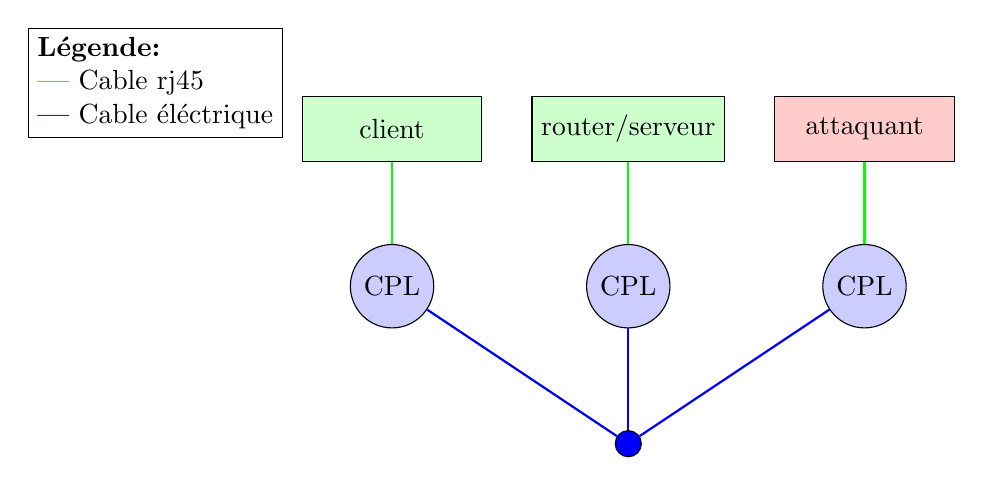
\begin{tikzpicture}[
      cpl/.style={
        draw,
        fill=blue!20,
        circle,
        minimum size= 1cm
      },
      pc/.style={
        draw,
        rectangle,
        fill=green!20,
        minimum width={width("router/serveur")+2pt},
        minimum height={height("/")+16pt},
      }
      ]
        \node[cpl] (cpl1) at (0,0) {CPL};
        \node[pc] (pc1) at (0,2) {client};
        \draw[-, thick, green] (cpl1) -- node[midway, above] {} (pc1);

        \node[cpl] (cpl2) at (3,0) {CPL};
        \node[pc] (pc2) at (3,2) {router/serveur};
        \draw[-, thick, green] (cpl2) -- node[midway, above] {} (pc2); 

        \node[cpl] (cpl3) at (6,0) {CPL};
        \node[pc, fill=red!20] (pc3) at (6,2) {attaquant};
        \draw[-, thick, green] (cpl3) -- node[midway, above] {} (pc3); 

        \node[circle, draw, fill=blue] (p) at (3,-2) {};
        \draw[-, thick, blue] (cpl1) -- node[midway, above] {} (p); 
        \draw[-, thick, blue] (cpl2) -- node[midway, above] {} (p); 
        \draw[-, thick, blue] (cpl3) -- node[midway, above] {} (p); 
      
        % Légende
        \node[draw, fill=white, above left=of cpl1, anchor=south east, yshift=0.5cm, text width=3cm] (legend) {
            \textbf{Légende:} \\
            \textcolor{green}{\textbf{---}} Cable rj45 \\
            \textcolor{blue}{\textbf{---}} Cable éléctrique 
        };
    \end{tikzpicture}
\end{figure}
=======
\paragraph{}Dans ce laboratoire, les trois ordinateurs sont connectés à des adaptateurs CPL, qui sont eux-mêmes connectés au réseau électrique isolé. Le premier ordinateur (S) est utilisé comme serveur, le deuxième ordinateur (C) est utilisé comme client et le troisième ordinateur (A) est utilisé comme attaquant. Les adaptateurs CPL permettent de transmettre les données entre les ordinateurs via le réseau électrique.

\section{Resultats des tests}
\paragraph{}Nous avons effectuer les different test présenté précedament dans notre laboratoire de test. Les résultats de ces tests sont présentés ci-dessous.

\subsection{Test de distribution des trames}
\paragraph{}Dans ce test, nous avons utilisé un logiciel de capture de paquets sur l'ordinateur attaquant pour observer la distribution des trames à travers le réseau CPL. 
\paragraph{}N'ayant pas capturé de trames, nous avons conclus que les trames n'étaient pas transmises par tous les adaptateurs CPL vers les ordinateurs, mais seulement aux ordinateurs qui étaient directement concernés (ici le serveur et le clients).

\subsection{Test d'interception des trames}
\paragraph{}Dans ce test, nous avons utilisé un logiciel de capture de paquets sur l'ordinateur attaquant pour tenter d'intercepter les trames échangées entre le serveur et le client. Nous avons également utilisé une commande pour effectuer du ARP spoofing afin de rediriger le trafic réseau vers l'ordinateur attaquant.
\paragraph{}Après avoir lancé le serveur HTTP sur l'ordinateur S et accédé à ce serveur depuis l'ordinateur C, nous avons pu capturer les trames échangées entre le serveur et le client. Les données capturées ont été analysées et nous avons pu constater que les trames étaient bien transmises entre le serveur et le client, mais que l'attaquant pouvait également intercepter ces trames grâce à l'ARP spoofing. Une attaque de type man-in-the-middle a donc pu être réalisée, permettant à l'attaquant de lire les données échangées entre le serveur et le client.

\section{Conclusion des tests}
\paragraph{}En conclusion, nos tests ont montré que les CPL se comportent de manière similaire aux réseaux Ethernet en ce qui concerne la distribution des trames et l'interception des données. Les trames ne sont pas diffusées à tous les adaptateurs CPL, mais seulement à ceux qui sont directement concernés par la communication. Cependant, il est possible d'intercepter les données échangées entre le serveur et le client en utilisant des techniques telles que l'ARP spoofing. Cela souligne l'importance de sécuriser les communications sur les réseaux CPL, tout comme sur les réseaux Ethernet traditionnels.

\section{Conclusion}





\appendix
\chapter{Definitions}
\paragraph{Signal numérique} Un signal numérique est une représentation discrète de données, généralement sous forme de bits (0 et 1). Contrairement aux signaux analogiques, qui peuvent prendre une infinité de valeurs, les signaux numériques n'ont que des valeurs spécifiques.
\paragraph{Signal analogique} Un signal analogique est une représentation continue de données, où les valeurs peuvent varier de manière fluide.
\paragraph{Modulation} La modulation est le processus de modification d'un signal porteur (généralement un signal sinusoïdal) pour transmettre des informations. Cela peut impliquer des changements dans l'amplitude, la fréquence ou la phase du signal porteur.




\paragraph{}Dans le cas des courants porteurs en ligne (CPL), la modulation est utilisée pour superposer les signaux numériques sur les signaux électriques existants dans les lignes électriques. Cela permet de transmettre des données à haut débit sur des infrastructures électriques existantes, sans nécessiter de câblage supplémentaire.
\chapter{Modulation du signal}

\paragraph{}La modulation du signal est la technique qui permet de transmettre des données numériques (0 ou 1) sur un support analogique. En clair, cela signifie qu'une suite de 0 et de 1 sont intégrées dans un signal sinusoïdal, ce qui permet de transmettre ces données sur un support qui ne peut pas transporter directement des signaux numériques. 

\section{Types de modulation}
Il existe plusieurs familles de modulation :
\begin{itemize}
    \item \textbf{Modulation d'Amplitude (AM)} : La force du signal est modifiée pour représenter les données.
    \item \textbf{Modulation de Fréquence (FM)} : La fréquence du signal est modifiée pour représenter les données.
    \item \textbf{Modulation de Phase (PM)} : La phase du signal est modifiée pour représenter les données.
\end{itemize}

\begin{figure}[ht]
    \centering
    \caption{Exemple de modulation d'amplitude, de fréquence et de phase}
    \label{fig:modulation_example}
    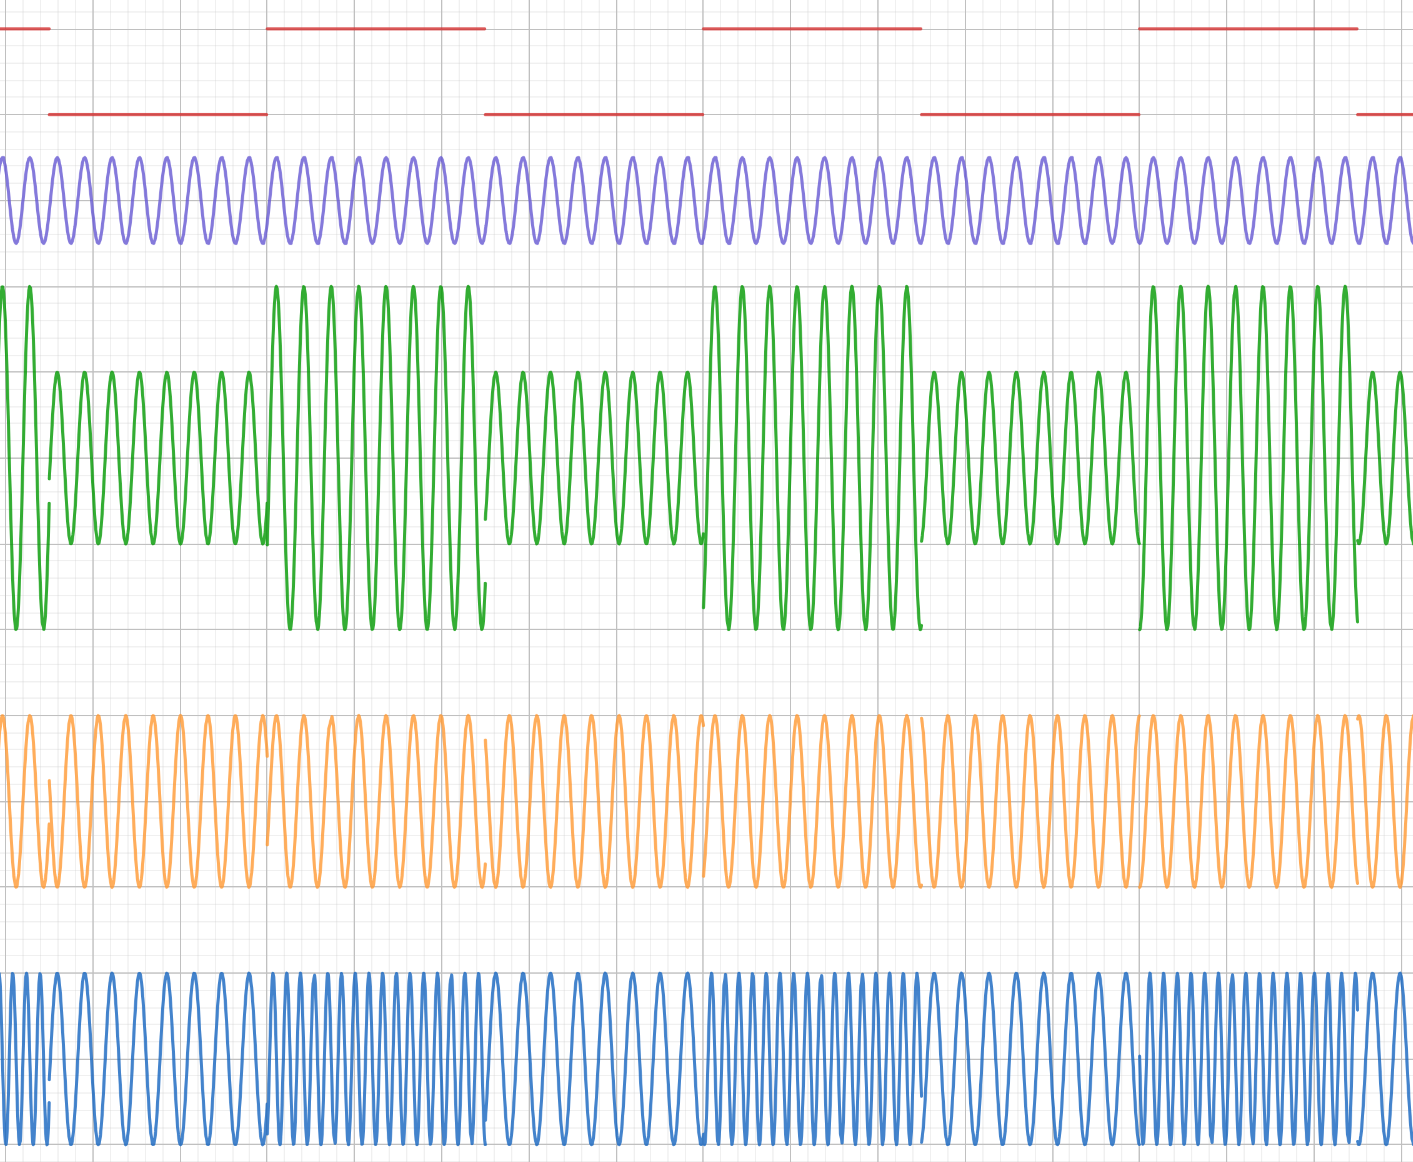
\includegraphics[scale=0.25]{images/ModulationExemple.png}
\end{figure}

\subsection{Modulation d'Amplitude (AM)}
\paragraph{}Dans la modulation d'amplitude, l'amplitude du signal porteur est modifiée en fonction de l'information à transmettre. Par exemple, un signal numérique peut être représenté par deux niveaux d'amplitude : un niveau élevé pour un bit "1" et un niveau bas pour un bit "0". Cette technique est simple mais sensible aux interférences et au bruit.
\paragraph{}Il existe plusieurs variantes de modulation d'amplitude :
\begin{itemize}
    \item \textbf{Modulation d'Amplitude (AM)} : La forme de base où l'amplitude du signal porteur est modifiée proportionnellement à l'amplitude du signal modulant.
    \item \textbf{Modulation d'Amplitude en Quadrature (QAM)} : Combine deux signaux modulés en amplitude pour transmettre plus d'informations, souvent utilisée dans les communications numériques.
    \item \textbf{Amplitude Shift Keying (ASK)} : Une forme de modulation numérique où les données binaires sont transmises en modifiant l'amplitude du signal porteur entre deux niveaux, la modulation est effectuée un ensemble discret de valeurs.
\end{itemize}
\paragraph{}La modulation d'amplitude est couramment utilisée dans les transmissions radio AM et dans certaines applications de communication numérique. Cependant, elle est moins résistante au bruit et aux interférences, ce qui peut entraîner une dégradation du signal.

\subsection{Modulation de Fréquence (FM)}
\paragraph{}Dans la modulation de fréquence, la fréquence du signal porteur est modifiée en fonction de l'information à transmettre. Cela permet de transmettre des données avec une meilleure résistance au bruit par rapport à la modulation d'amplitude. Par exemple, un bit "1" peut être représenté par une fréquence plus élevée, tandis qu'un bit "0" est représenté par une fréquence plus basse. 
\paragraph{}Il existe plusieurs variantes de modulation de fréquence : 
\begin{itemize}
    \item \textbf{Modulation de Fréquence (FM)} : La forme de base où la fréquence instantanée de la porteuse varie proportionnellement à l'amplitude du signal modulant.
    \item \textbf{Modulation par saut de fréquence (FSK)} : Utilisée dans les communications numériques, la FSK est une forme de modulation de fréquence où les données binaires sont transmises en changeant la fréquence de la porteuse entre un ensemble discret de valeurs.
    \item \textbf{Minimum-Shift Keying (MSK)} : Une forme de FSK continue-phase où les changements de fréquence se produisent aux croisements de zéro du signal, ce qui minimise l'occupation spectrale.
\end{itemize}
\paragraph{}La modulation de fréquence est souvent utilisée dans les transmissions radio et audio. Cette technique est particulièrement efficace pour les communications à longue distance, car elle réduit les effets des interférences et du bruit.

\subsection{Modulation de Phase (PM)}
\paragraph{}Dans la modulation de phase, la phase du signal porteur est modifiée en fonction de l'information à transmettre. Par exemple, un bit "1" peut être représenté par un décalage de phase de 180 degrés, tandis qu'un bit "0" reste inchangé. Cette technique est moins courante que la modulation d'amplitude et de fréquence, mais elle est utilisée dans certaines applications spécifiques.
\begin{itemize}
    \item \textbf{Modulation de Phase (PM)} : La forme de base où la phase du signal porteur est modifiée proportionnellement à l'amplitude du signal modulant.
    \item \textbf{Phase Shift Keying (PSK)} : Une forme de modulation numérique où les données binaires sont transmises en changeant la phase du signal porteur entre un ensemble discret de valeurs.
    \item \textbf{Quadrature Phase Shift Keying (QPSK)} : Une forme avancée de PSK qui permet de transmettre deux bits par symbole en utilisant quatre phases différentes.
    \item \textbf{Differential Phase Shift Keying (DPSK)} : Une variante de PSK où la phase du signal est modifiée par rapport à la phase du symbole précédent, ce qui permet une meilleure résistance aux erreurs de phase.
\end{itemize}
\paragraph{}La modulation de phase est souvent utilisée dans les systèmes de communication numériques, où elle peut offrir une meilleure efficacité spectrale et une résistance accrue aux interférences. Elle est également utilisée dans des technologies telles que le Wi-Fi et le Bluetooth, où la qualité du signal est cruciale.

\subsection{Combinaison de modulations}
\paragraph{}Enfin, il est important de noter que ces techniques de modulation peuvent etre combiner pour former des systèmes de modulation plus complexes. Par exemple, la modulation d'amplitude en quadrature (QAM) combine la modulation d'amplitude et la modulation de phase pour transmettre plusieurs bits par symbole, ce qui augmente l'efficacité spectrale. De même, la modulation de fréquence en quadrature (QFM) combine la modulation de fréquence et la modulation de phase pour améliorer la robustesse du signal.

\section{Encodage des données}

\paragraph{}L'encodage des données est le processus de conversion des données numériques en un format qui peut être transmis sur un support analogique. Par exemple, un chiffre decimal est encodé en binaire, puis en un signal analogique à l'aide de techniques de modulation.
\paragraph{}Dans la majorité des systèmes de communication, les données numériques sont d'abord converties en binaire, puis les bits sont regroupés en symboles. Chaque symbole peut représenter un ensemble de bits, et la modulation est utilisée pour convertir ces symboles en signaux analogiques. Par exemple, dans la modulation d'amplitude en quadrature (QAM), chaque symbole peut représenter plusieurs bits, ce qui permet une transmission plus efficace des données.
\paragraph{}L'utilisation de symboles permet de réduire la complexité de la transmission et d'augmenter l'efficacité spectrale. Par exemple, dans le cas de la modulation QAM, chaque symbole peut représenter 2, 4, 8, ou même 16 bits, en fonction du nombre de niveaux d'amplitude et de phase utilisés. Cela permet de transmettre plus d'informations en utilisant moins de bande passante.

\end{document}
